\chapter{Introduction}
This research was inspired by learning about the power and capabilities of applying usage data collected by mobile apps in extremely popular real-world mobile apps in the early days of mobile apps (before Android, iOS and other modern mobile platforms were released). 
Several years later, when consulting with another company with over ten million active users I discovered they had included two analytics tools in their apps where there were numerous discrepancies in the data collected, the ways the counted and the resulting reports, yet they were both considered necessary. The engineers then added a third analytics library in the hope it would correlate with one or other of the existing libraries - it didn't, instead it had distinct characteristics and counts. And yet the developers were able to discover how their apps were used in incredible detail and by applying what they learned their apps became increasingly popular and financially successful.

These experiences led me to starting my PhD in order to research the potential of mobile analytics, and to understand some of their flaws and the effects of those flaws. During my research there have been incredible changes in the mobile landscape (for instance major manufacturers, operating systems, etc. have appeared, mushroomed, and disappeared). Similarly many test automation tools and frameworks have been and gone. Meanwhile, apps and app stores have spread beyond smartphones and tablets to desktop operating systems, cloud-based product offerings such as Salesforce, etc. Google's Android platform includes platform-level data collection, reporting and analytics intended to help developers learn about ways they can improve their apps. Meanwhile regulation has started to emphasise and highlight some of the many risks and concerns with gathering data wantonly. 

Despite all these changes, and my limited inroads into a subset of the entire landscape, the research seems to indicate the potential of applying usage analytics to improve both the product (the software) and the process (how the software is developed and tested). The research also identified flaws within analytics tools and also between analytics tools. Both the potential and the flaws appear worth sharing with researchers and with practitioners to help them chose and use analytics wisely.

\section{My contributions in this thesis}
I have introduced the concept of using mobile analytics to help illuminate emergent behaviours of mobile apps and set mobile analytics into a broader context of other sources and reflections of perceived quality of mobile apps.

I have contributed the first studies into Platform Analytics as provided by Google Play Console, including pre-launch reports and Android Vitals, services intended to help developers identify quality issues with their Android apps in order to address these issues so they do not affect end-users. I have helped demonstrate their efficacy, despite various flaws I also discovered, identified and reported to Google. 

\begin{figure}[ht]
    \centering
    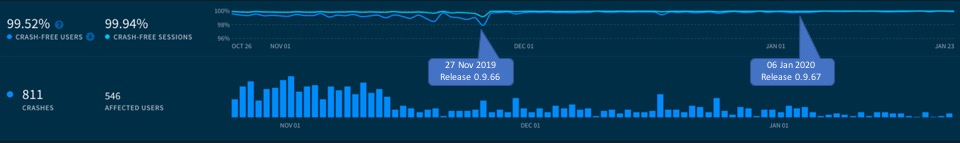
\includegraphics[width=\textwidth]{images/annotated_pocketcode_90_day_fabric_crashlytics_report.jpg}
    \caption{Pocket Code improvements in crash rate, in 90 days}
    %\Description{Pocket Code: When the project team investigated crashes they improved the reliability}
    \label{fig:pocketcode_improvements_in_crash_rate}
\end{figure}

Through my work with one the Catrobat project team, as Figure \ref{fig:pocketcode_improvements_in_crash_rate} shows, within 90 days and 2 releases we were were able to tame their key Android app's crash rate that was previously precariously high. The team had not been able to address the crash rate despite applying many of the recognised and recommended software development practices.

I also compare Crashlytics reports with the Platform Analytics and again identify both internal and cross-tool flaws and inconsistencies. Some of these have already been reported to Google in preparation for a full report to be submitted on completion of some ongoing research.

\begin{figure}[ht]
    \centering
    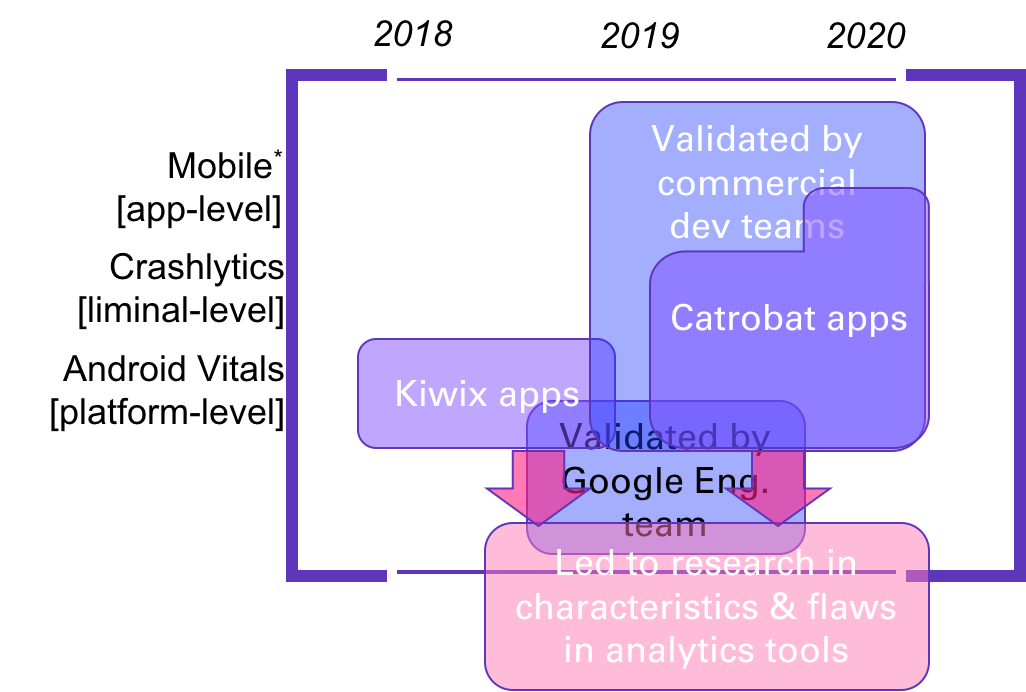
\includegraphics[width=10cm]{images/visual-connections-in-research.png}
    \caption{Visual Connections in my research}
    \label{fig:visual-connections-in-research}
\end{figure}

Figure \ref{fig:visual-connections-in-research} aims to provide a visual overlay of the main practical elements of the research. The practical research  

I instigated and led the development of several opensource software utilities to help record and preserve reports and underlying failure data from Google Play Console and Android Vitals. We have successfully extended the capabilities of the utilities and further extensions are practical. Research benefits:
\begin{itemize}
    \item Evidence preserved for analysis:
    \item Data can now be compared and further assessed:
    \item Data and contents can be shared by developers of Android apps with other researchers - extending the body of knowledge about crashes (un-reliability) and ANRs (run-time unresponsiveness). \emph{bringing previously unknown data, practices and tools into the open so others can understand them, make more informed decisions, and perform further research.}
\end{itemize}

I made data available for further research based on data originally only made available to app developers.

The research has been presented at various conferences and workshops, including at NII Shonan: "Release Engineering for Mobile Applications". 

\section{Outline of this thesis}
Bugs are ubiquitous in software (c.f. even Knuth's challenge was met) and self-aware developers expect there will be bugs in their software. 

Even top development teams are likely to learn of bugs they were not able to find, and cannot reproduce. For instance, Google's Android Auto Team have asked for help from end users to identify patterns that may help the team find and address the bug~\footnote{\url{https://support.google.com/androidauto/thread/2865341?msgid=44437416}}. As reported by \texttt{autoevolution} in May 2020:  
\emph{"As it turns out, the Android Auto team wasn’t able to reproduce the whole thing, so it’s now asking users to send additional reports with more information to help fix the problem."}~\footnote{~\url{https://www.autoevolution.com/news/google-wants-users-to-help-fix-widespread-android-auto-bug-143760.html}}.

Developers want and need to know how well their apps are performing from various perspectives such as: growth and adoption (\emph{``do we have more users and are they using the app [more] often?"}), users' ratings and reviews (\emph{``do they like our work?"} and in terms of quality (\emph{``does it perform well? is it fast and reliable?"}). Google's Google Play app store provides developers with answers to all these niggling questions through a developer-oriented user interface called Google Play Console. 
In Google Play Console they provide various tools, reports and data all aimed at informing developers about how their apps are 'doing' and performing. Broadly, these include an overview page with one line of pre-selected data per app managed by the developer account. (\emph{TODO perhaps I should explain this concept of developer account e.g. in the glossary?} Then, per app, Google provides an overview dashboard of graphs \emph{TODO add screenshot?} which, in turn, link to more detailed reports and information which provide greater depth. Some graphs only appear when Google's algorithms decide they are relevant, these seem to be related to events and/or volumes of underlying data.

Chapter TBD provides details of my understanding of how Google collects the underlying data (they do not document, explain or encourage research in how their system works, We return to their behaviour and the effects later in this introduction). And chapter TBD describes software we developed to help collect data from Google Play Console in order to facilitate both research and to enable developers to collect and use data...

Crashes are often considered a concrete measure of poor performance of software and there has been extensive research in crashes for Android applications, in particular. I suspect there are various reasons for the focus on crashes as an oracle for testing software, crashes are unambiguous (even if the causes are not) and they are also binary so easy to determine whether software has, or has not, crashed. 

Google launched a service called Android Vitals as a new, intrinsic part of Google Play Console in 2016/17 \emph{TODO confirm the date and revise this sentence} where they popularised a measure called \emph{Stability} to assess the quality of Android apps. Their measure includes both crashes and when an application freezes or is unresponsive for at least 5 seconds from a user's perspective, a term Google call Application Not Responding (ANR).

\subsection{Analogue and Digital Feedback}
Feedback can help developers to find and choose ways to improve their software. Various researchers have investigated way to understand and use feedback provided by end-users, for instance, in ratings and reviews users provide to the app store. For the purposes of my research I term feedback people provide as \emph{analogue feedback} as it has the richness and complexity of analogue signals, and also challenges of processing and comprehension.

In contrast, digital feedback originates from software and is generally deterministic~\footnote{~\url{https://en.wiktionary.org/wiki/deterministic}}. For the purposes of my research I consider digital feedback as that provided by running software where programmers added code to programs to collect data that provides feedback about software use and certain behaviours of that software. The addition of the code may be automated, in part, or wholly, for instance by another program or script. As an example, AppPulse Mobile claims they can add analytics automatically without developers writing a line of code~\footnote{~\url{https://www.microfocus.com/en-us/products/apppulse-mobile-app-apm-monitoring/overview}}.


% Mobile Developer's Guide to the fifth dimension
% available from https://www.dropbox.com/s/no70z2hiod6z7o8/Fifth_Dimension_v1.pdf?dl=0 (took 20 - 30 mins to track down)

\subsection{The Reaper Cometh}
AppBrain is a business that actively monitors and reports on Android Apps in the Google Play Store. The business was founded by two ex-Google engineers, as I am. They state Google is actively culling Android apps from the Google Play store and estimate approximately 16\% of apps are \emph{"low quality apps"} and \emph{"unlikely to be useful"}~\footnote{\url{https://www.appbrain.com/stats/number-of-android-apps}} % Percentage of low quality apps: 16%


\subsection{Validation of the concepts}
My practical research focuses on two sets of Android applications, those of the Kiwix and Catrobat project teams. According to data and reports Google provides the development teams their active user-bases are 362,595 for the Kiwix project across 18 published apps, and 148,966 for the Catrobat project across 6 published apps. %data obtained on 16th May 2020.
TODO map these apps to the buckets in the table from the 'beyond Google Play' paper.

While these apps include a useful variety of user populations (from 10's of users to 150K+ across many countries and tens of apps) they could be perceived as a \emph{drop in the ocean} of the millions of apps currently available in the Google Play app store. Also, both project teams are non commercial, and may have different working dynamics from commercial development projects and teams. As my research was inspired from my consulting work with businesses who rely on the success of their apps I chose to supplement these two projects by engaging with developers from several commercial development teams. These include: Moonpig, Moodspace, and LocalHalo. Each values and uses analytics data during their development process to assess post-launch issues with their apps. From time to time things go awry with the behaviours of one or more of their releases and analytics helps them to identify and respond to issues before they become pervasive. For the LocalHalo app, \emph{TODO add details}... For Moonpig \emph{TODO add details}...

\subsubsection{Validation by the Google Engineering Team}
In Spring 2019 I reported various flaws or potential anomalies in various reports Google Play Console provides to developers to the then Product Manager for Android Vitals, Mr Fergus Hurley. As the long-term product owner he has extensive and insider experience of the tools and reports Google provides to an estimated population of over 1 million Android developers \emph{TODO add references e.g. to the Beyond Google Play paper and the one about a few developers creating an exponential number of apps}. I asked for his perspective during both a long in-person meeting and a follow-up video call a few weeks later. He confirmed several of the issues and debated others. He was willing to go on record in one of my accepted peer-reviewed papers on the topic \emph{TODO add link} and asked me to continue to share my findings with them. During the next 12 months he and then they added more Google staff to the discussion and asked me to write up my findings in a document that became over 30 pages long. Their policy means they are unlikely to confirm changes they make as a result of my research and findings, nonetheless they accept and value the feedback that has been provided. They also confirmed various bugs were ones they want to address.
